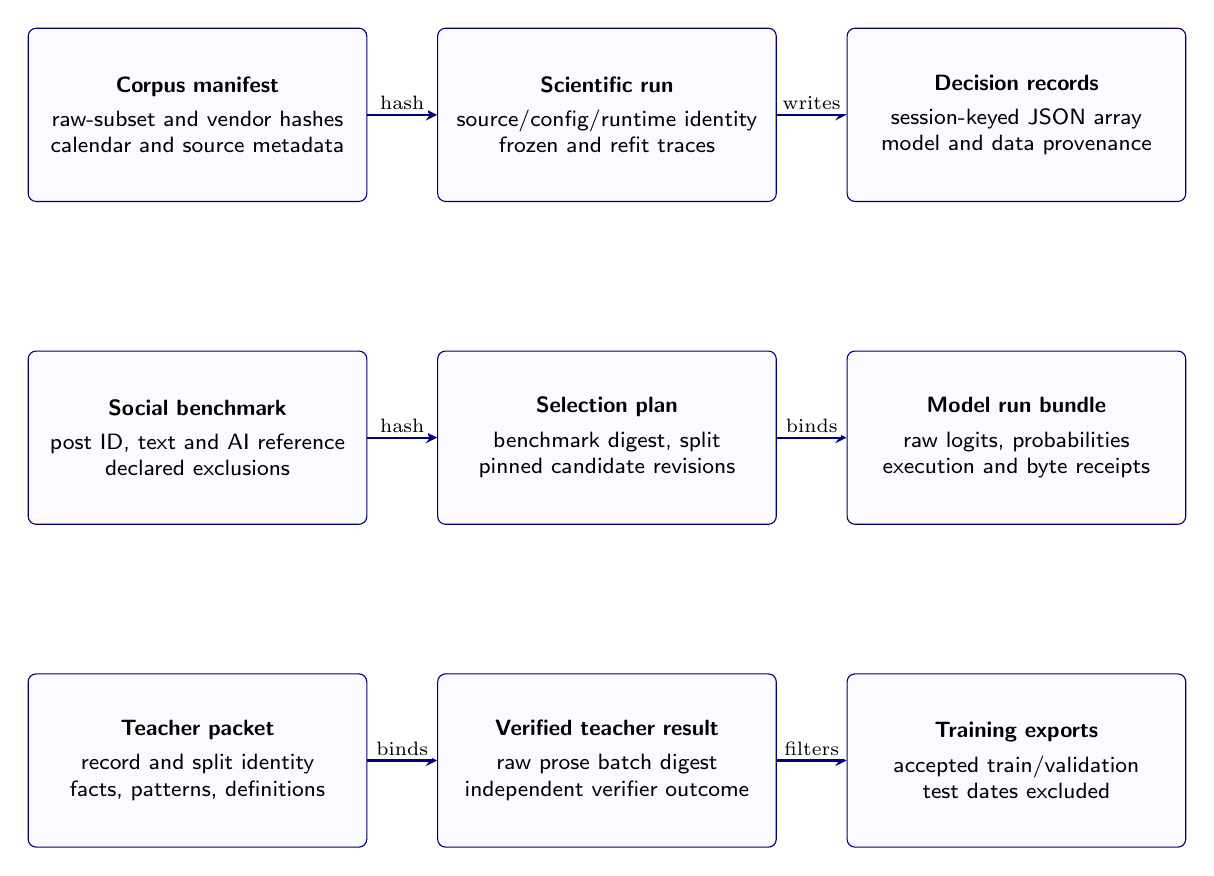
\begin{tikzpicture}[x=1mm,y=1mm,box/.style={draw=blue!45!black,fill=blue!2,rounded corners=1mm,align=center,text width=39mm,minimum height=22mm,inner sep=2mm,font=\sffamily\footnotesize},link/.style={->,>=stealth,draw=blue!50!black,thick}]
\node[box] (manifest) at (23,105) {\textbf{Corpus manifest}\\[1mm]raw-subset and vendor hashes\\calendar and source metadata};
\node[box] (run) at (75,105) {\textbf{Scientific run}\\[1mm]source/config/runtime identity\\frozen and refit traces};
\node[box] (records) at (127,105) {\textbf{Decision records}\\[1mm]session-keyed JSON array\\model and data provenance};
\node[box] (benchmark) at (23,64) {\textbf{Social benchmark}\\[1mm]post ID, text and AI reference\\declared exclusions};
\node[box] (plan) at (75,64) {\textbf{Selection plan}\\[1mm]benchmark digest, split\\pinned candidate revisions};
\node[box] (bundle) at (127,64) {\textbf{Model run bundle}\\[1mm]raw logits, probabilities\\execution and byte receipts};
\node[box] (packet) at (23,23) {\textbf{Teacher packet}\\[1mm]record and split identity\\facts, patterns, definitions};
\node[box] (teacher) at (75,23) {\textbf{Verified teacher result}\\[1mm]raw prose batch digest\\independent verifier outcome};
\node[box] (exports) at (127,23) {\textbf{Training exports}\\[1mm]accepted train/validation\\test dates excluded};
\draw[link] (manifest.east) -- (run.west) node[pos=.5,above,fill=white,inner sep=.5mm,font=\scriptsize]{hash};
\draw[link] (run.east) -- (records.west) node[pos=.5,above,fill=white,inner sep=.5mm,font=\scriptsize]{writes};
\draw[link] (benchmark.east) -- (plan.west) node[pos=.5,above,fill=white,inner sep=.5mm,font=\scriptsize]{hash};
\draw[link] (plan.east) -- (bundle.west) node[pos=.5,above,fill=white,inner sep=.5mm,font=\scriptsize]{binds};
\draw[link] (packet.east) -- (teacher.west) node[pos=.5,above,fill=white,inner sep=.5mm,font=\scriptsize]{binds};
\draw[link] (teacher.east) -- (exports.west) node[pos=.5,above,fill=white,inner sep=.5mm,font=\scriptsize]{filters};
\end{tikzpicture}
